\documentclass[figures_tabs.tex]{subfiles}
\begin{document}
\section{Figures \& Tables} % (fold)
\label{sec:figures_tables}
\begin{table}[H]
    \centering
    \begin{tabularx}{\textwidth}{|l|X|}
        \hline
        Field & Description \\
        \hline
        AppID & The application ID. \\
        \hline
        Name & The name of the game. \\
        \hline
        Developer & A comma separated list of developers of the game. \\
        \hline
        Publisher & A comma separated list of publishers of the game. \\
        \hline
        Score Rank & The score rank of the game based on user reviews. A score
        rank of 75\% indicates that the game has better reviews than 75\% of
        Steam games. \\
        \hline
        \emph{Owners} & The estimated number of users who own the game. This
        figure can be inflated with free games or games being offered as a free
        weekend. \\
        \hline
        \emph{Players Forever} & The number of users who have played the game
        since March 2009. \\
        \hline
        \emph{Players 2 Weeks} & The number of users who have played the game in
        the two weeks period of this request. \\
        \hline
        Average Forever & Average playtime since March 2009 in minutes.\\
        \hline
        Average 2 Weeks & Average playtime in two weeks period in minutes. \\
        \hline
        Median Forever & Median playtime since March 2009 in minutes. \\
        \hline
        Median 2 Weeks & Median playtime in two weeks period in minutes. \\
        \hline
        CCU & The peak number of concurrent users playing the game the day
        before the request was made. \\
        \hline
        Price & The current price of the game in US cents. \\
        \hline
    \end{tabularx}
    \vspace{1ex}
    \caption{The dataset's fields}
    \label{table:fields}
\end{table}


\begin{figure}[H]
    \centering
    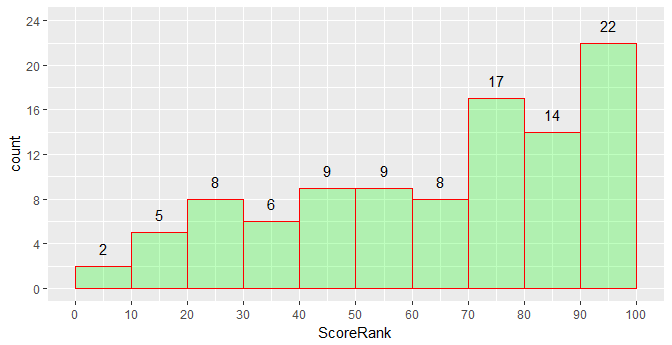
\includegraphics[width=\textwidth]{img/score_rank.png}
    \caption{Histogram of the score rank}
    \label{fig:score_rank}
\end{figure}

\begin{figure}[H]
    \centering
    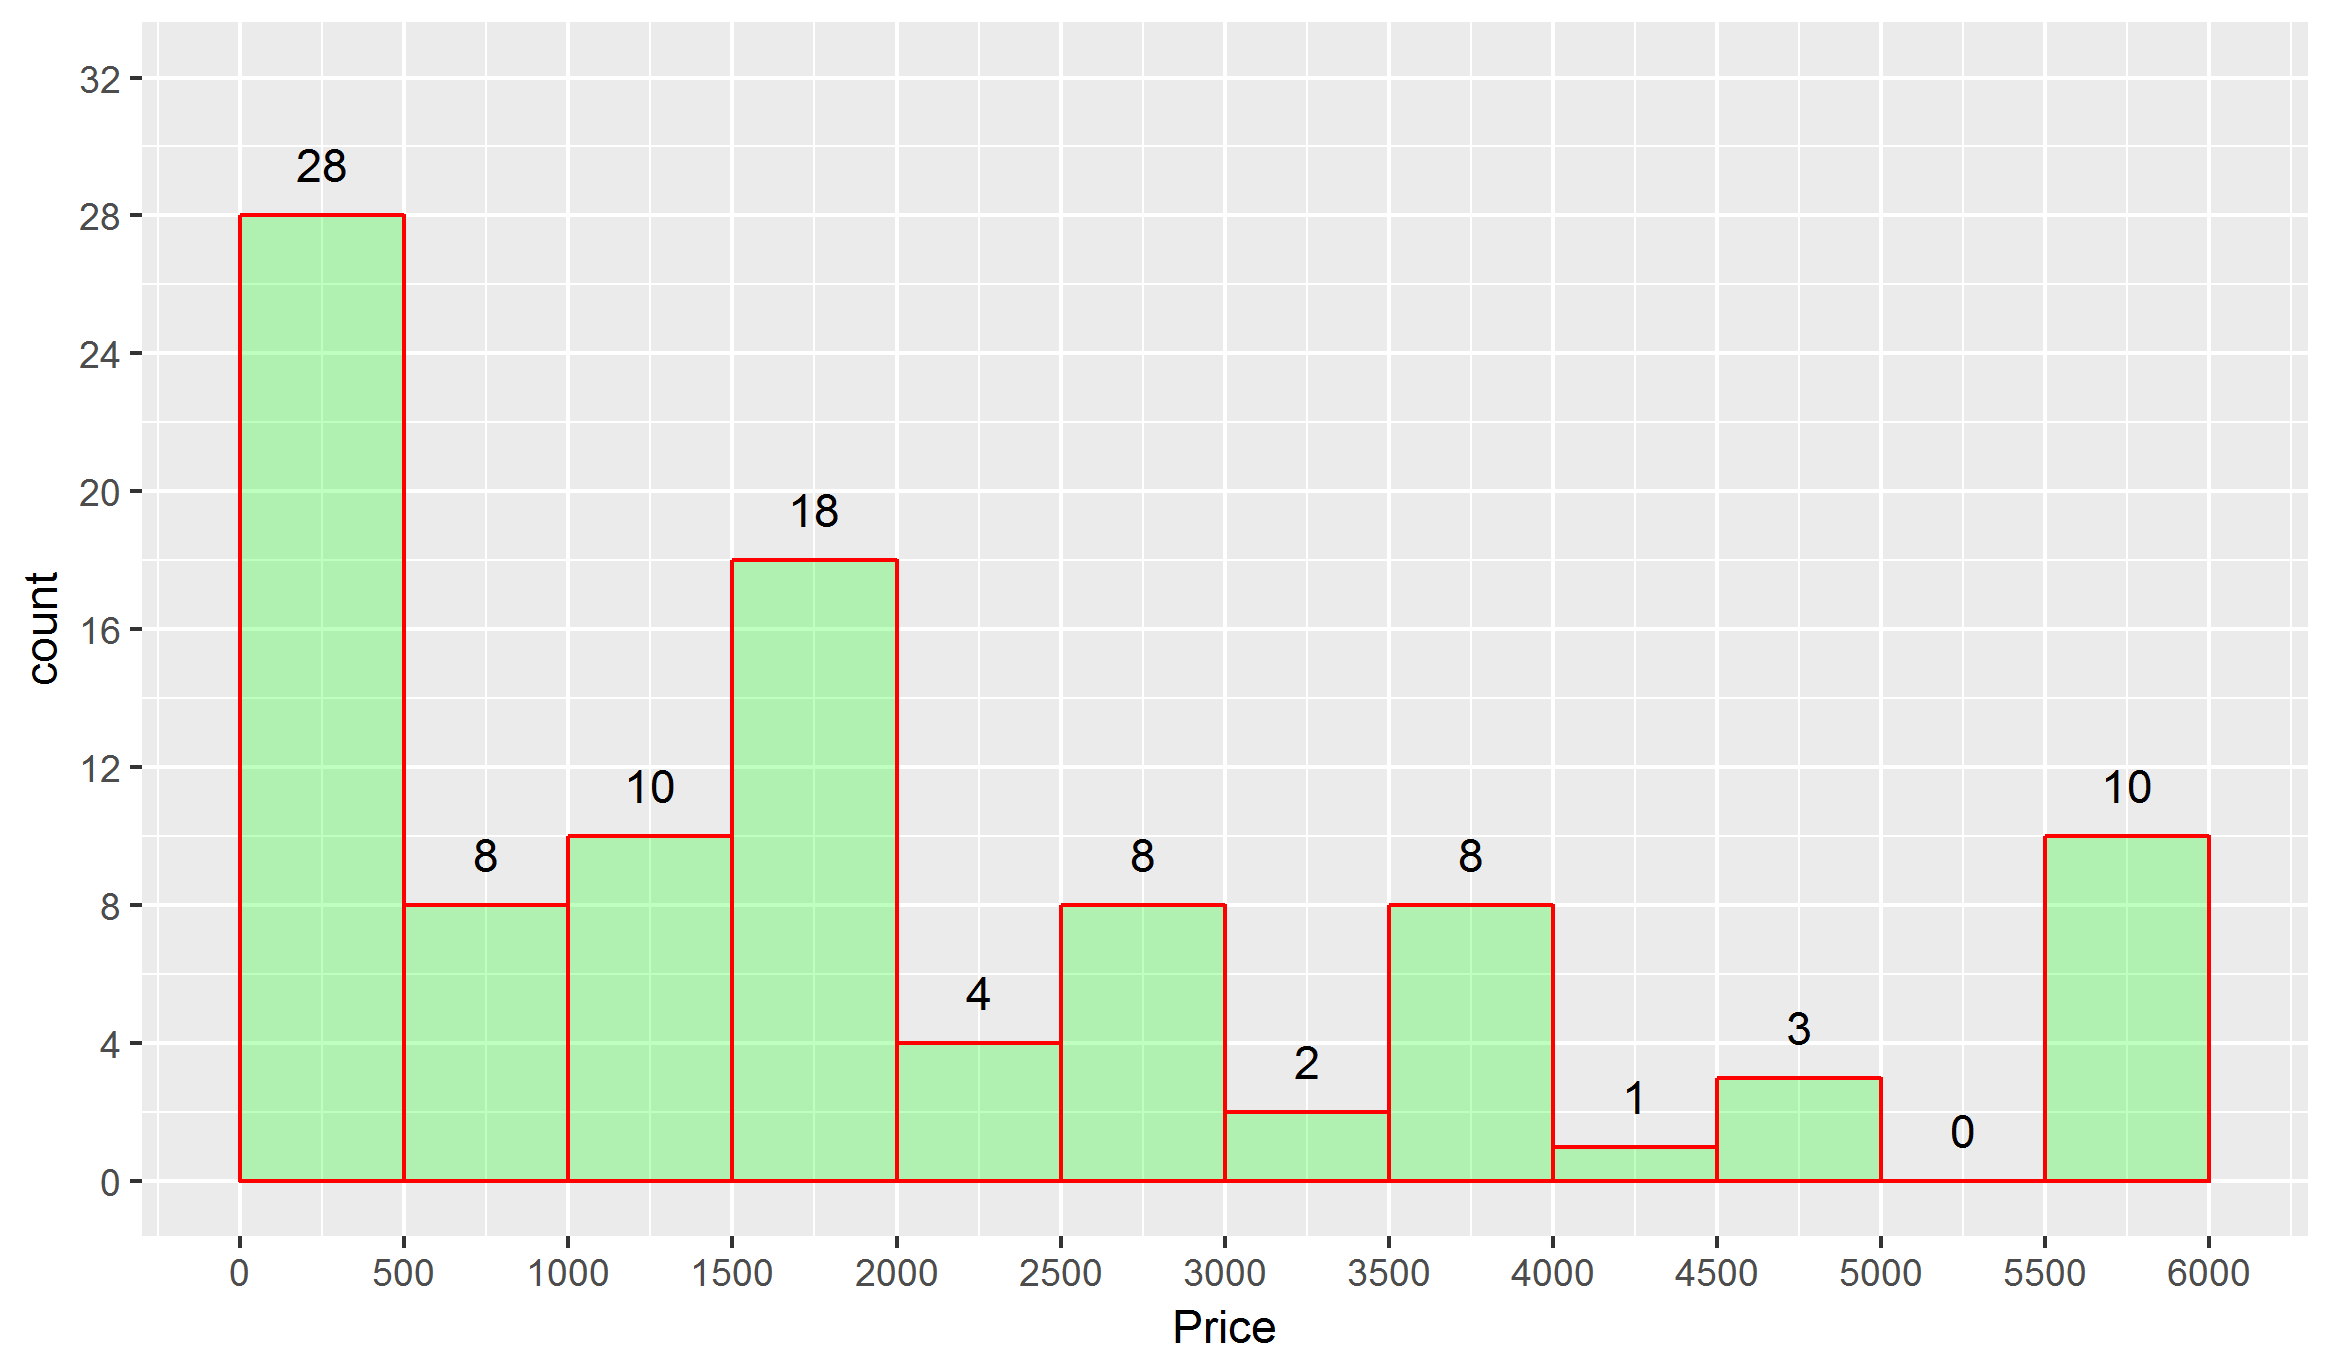
\includegraphics[width=\textwidth]{img/price.png}
    \caption{Histogram of the game prices}
    \label{fig:price}
\end{figure}

\begin{figure}[H]
    \centering
    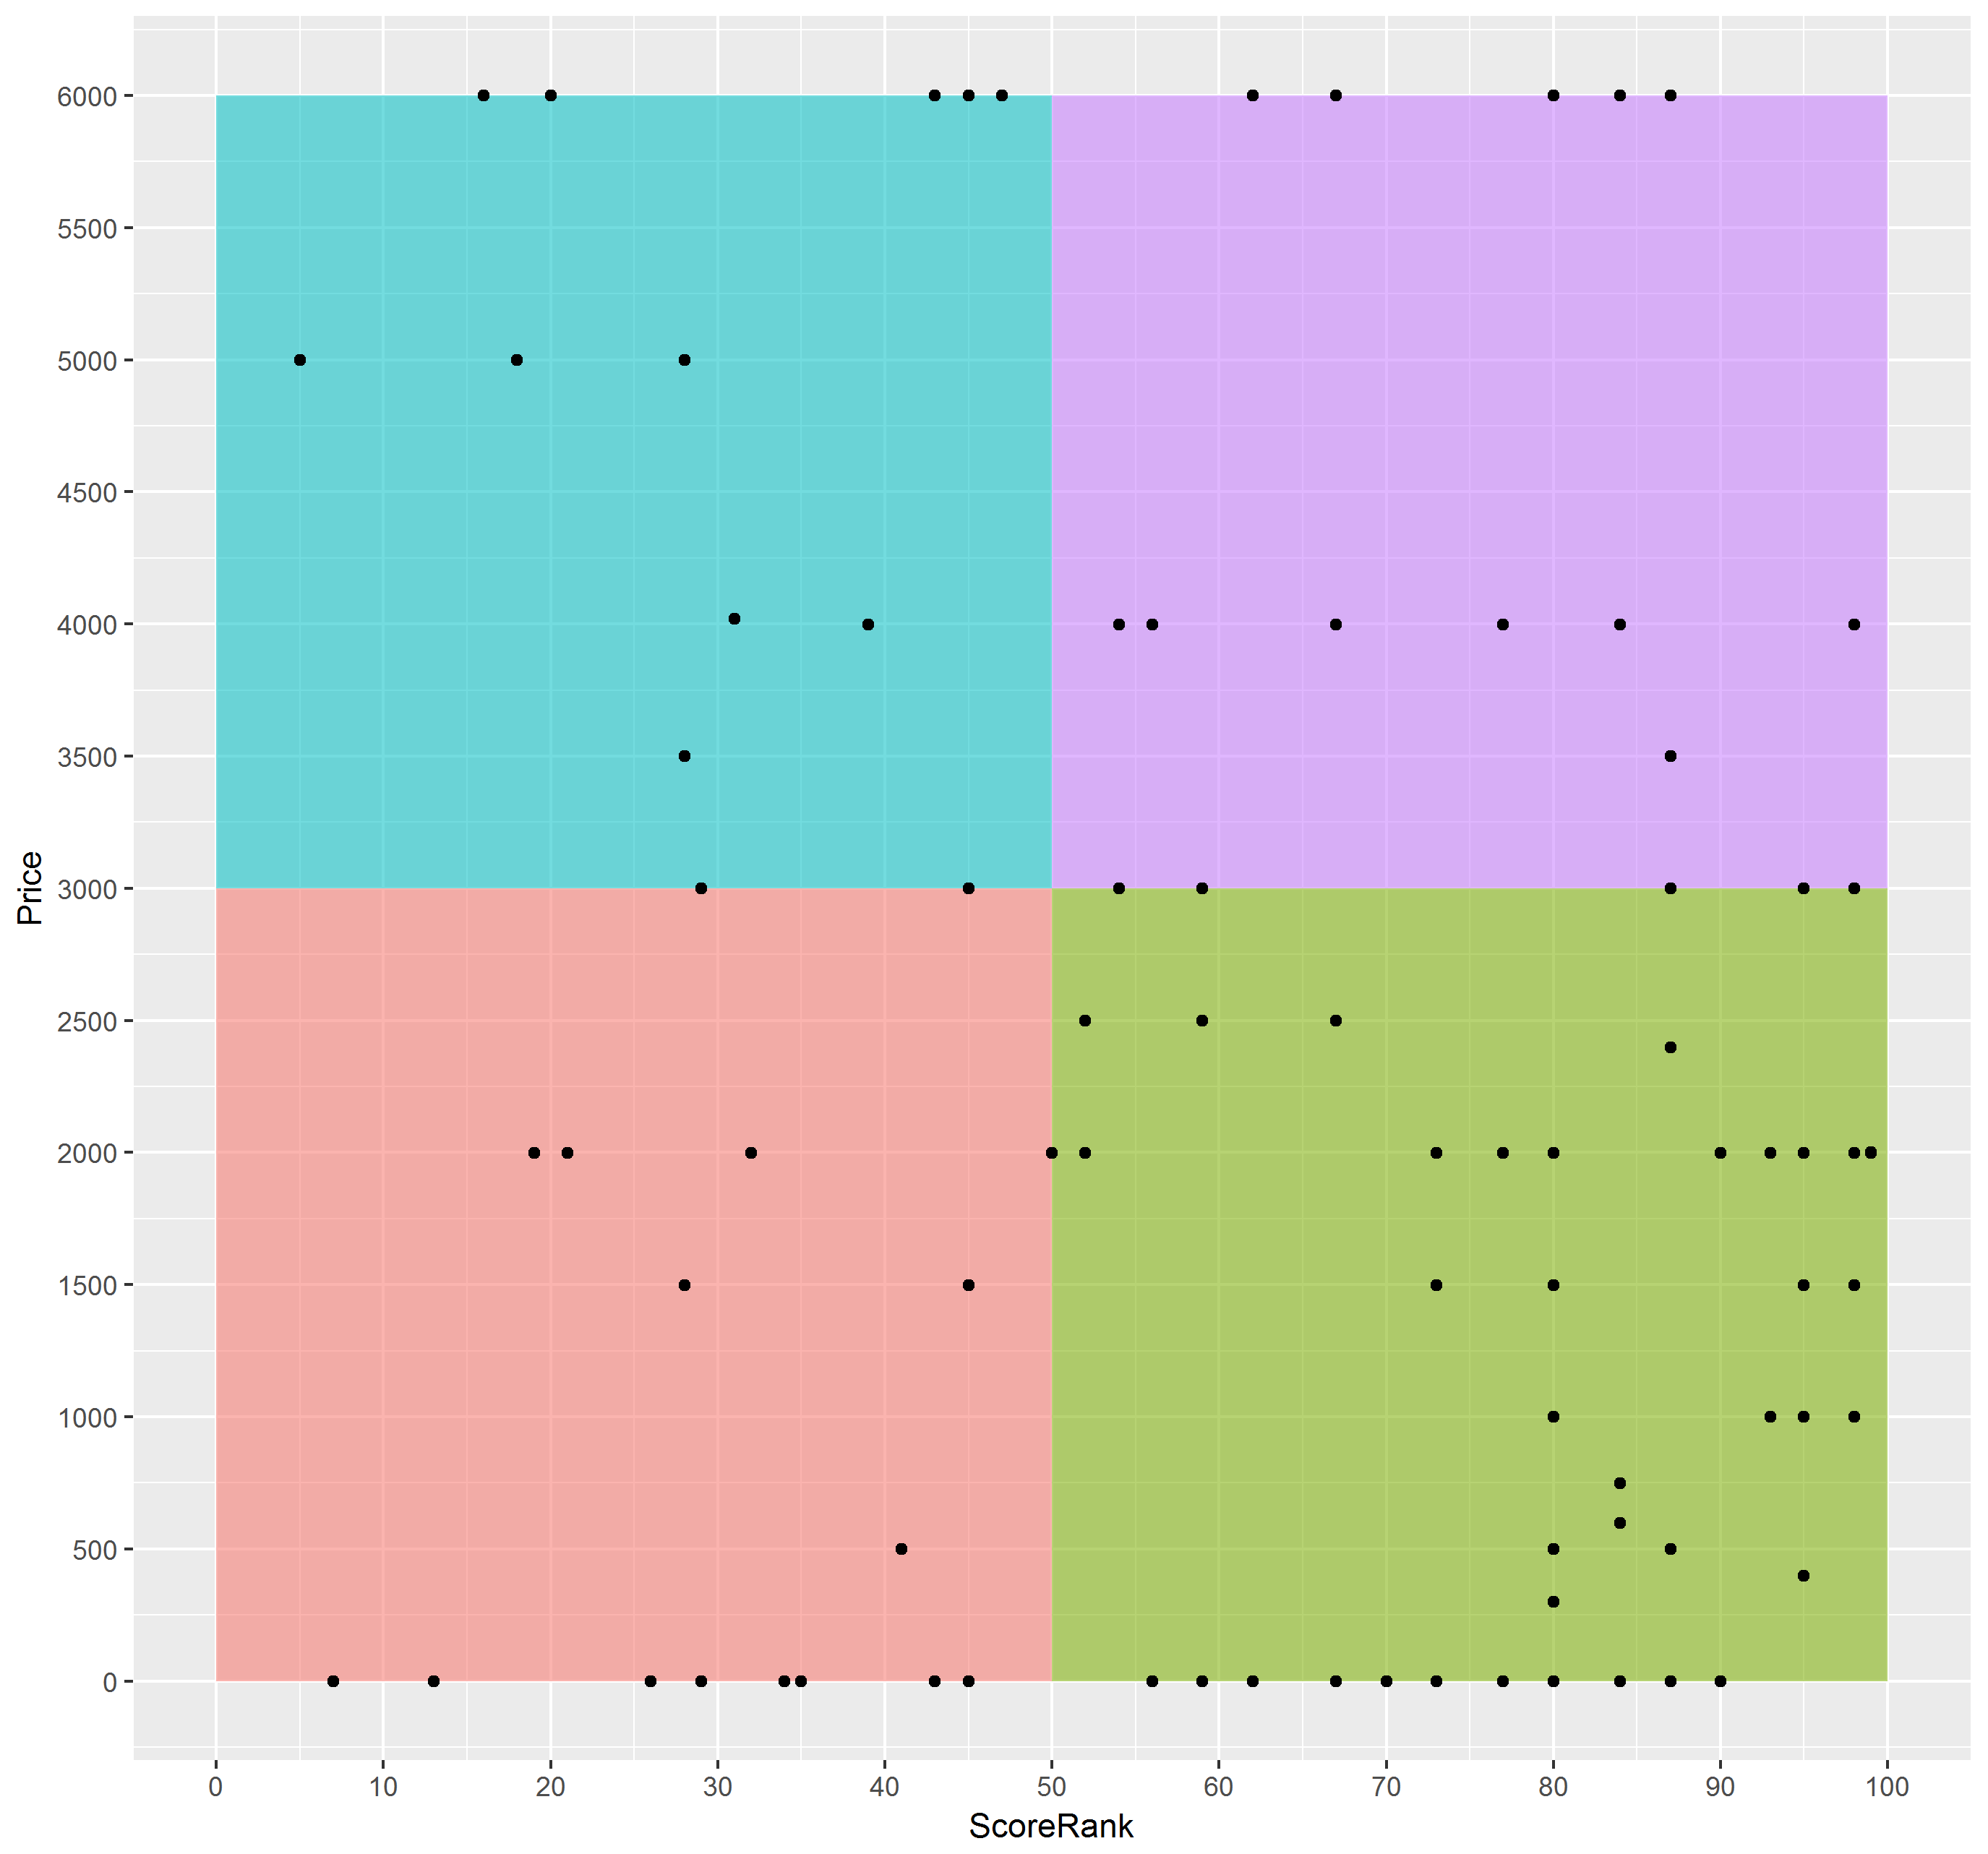
\includegraphics[width=\textwidth]{img/score_price.png}
    \caption{Plotting of price and score rank}
    \label{fig:score_price}
\end{figure}

\begin{figure}[H]
    \centering
    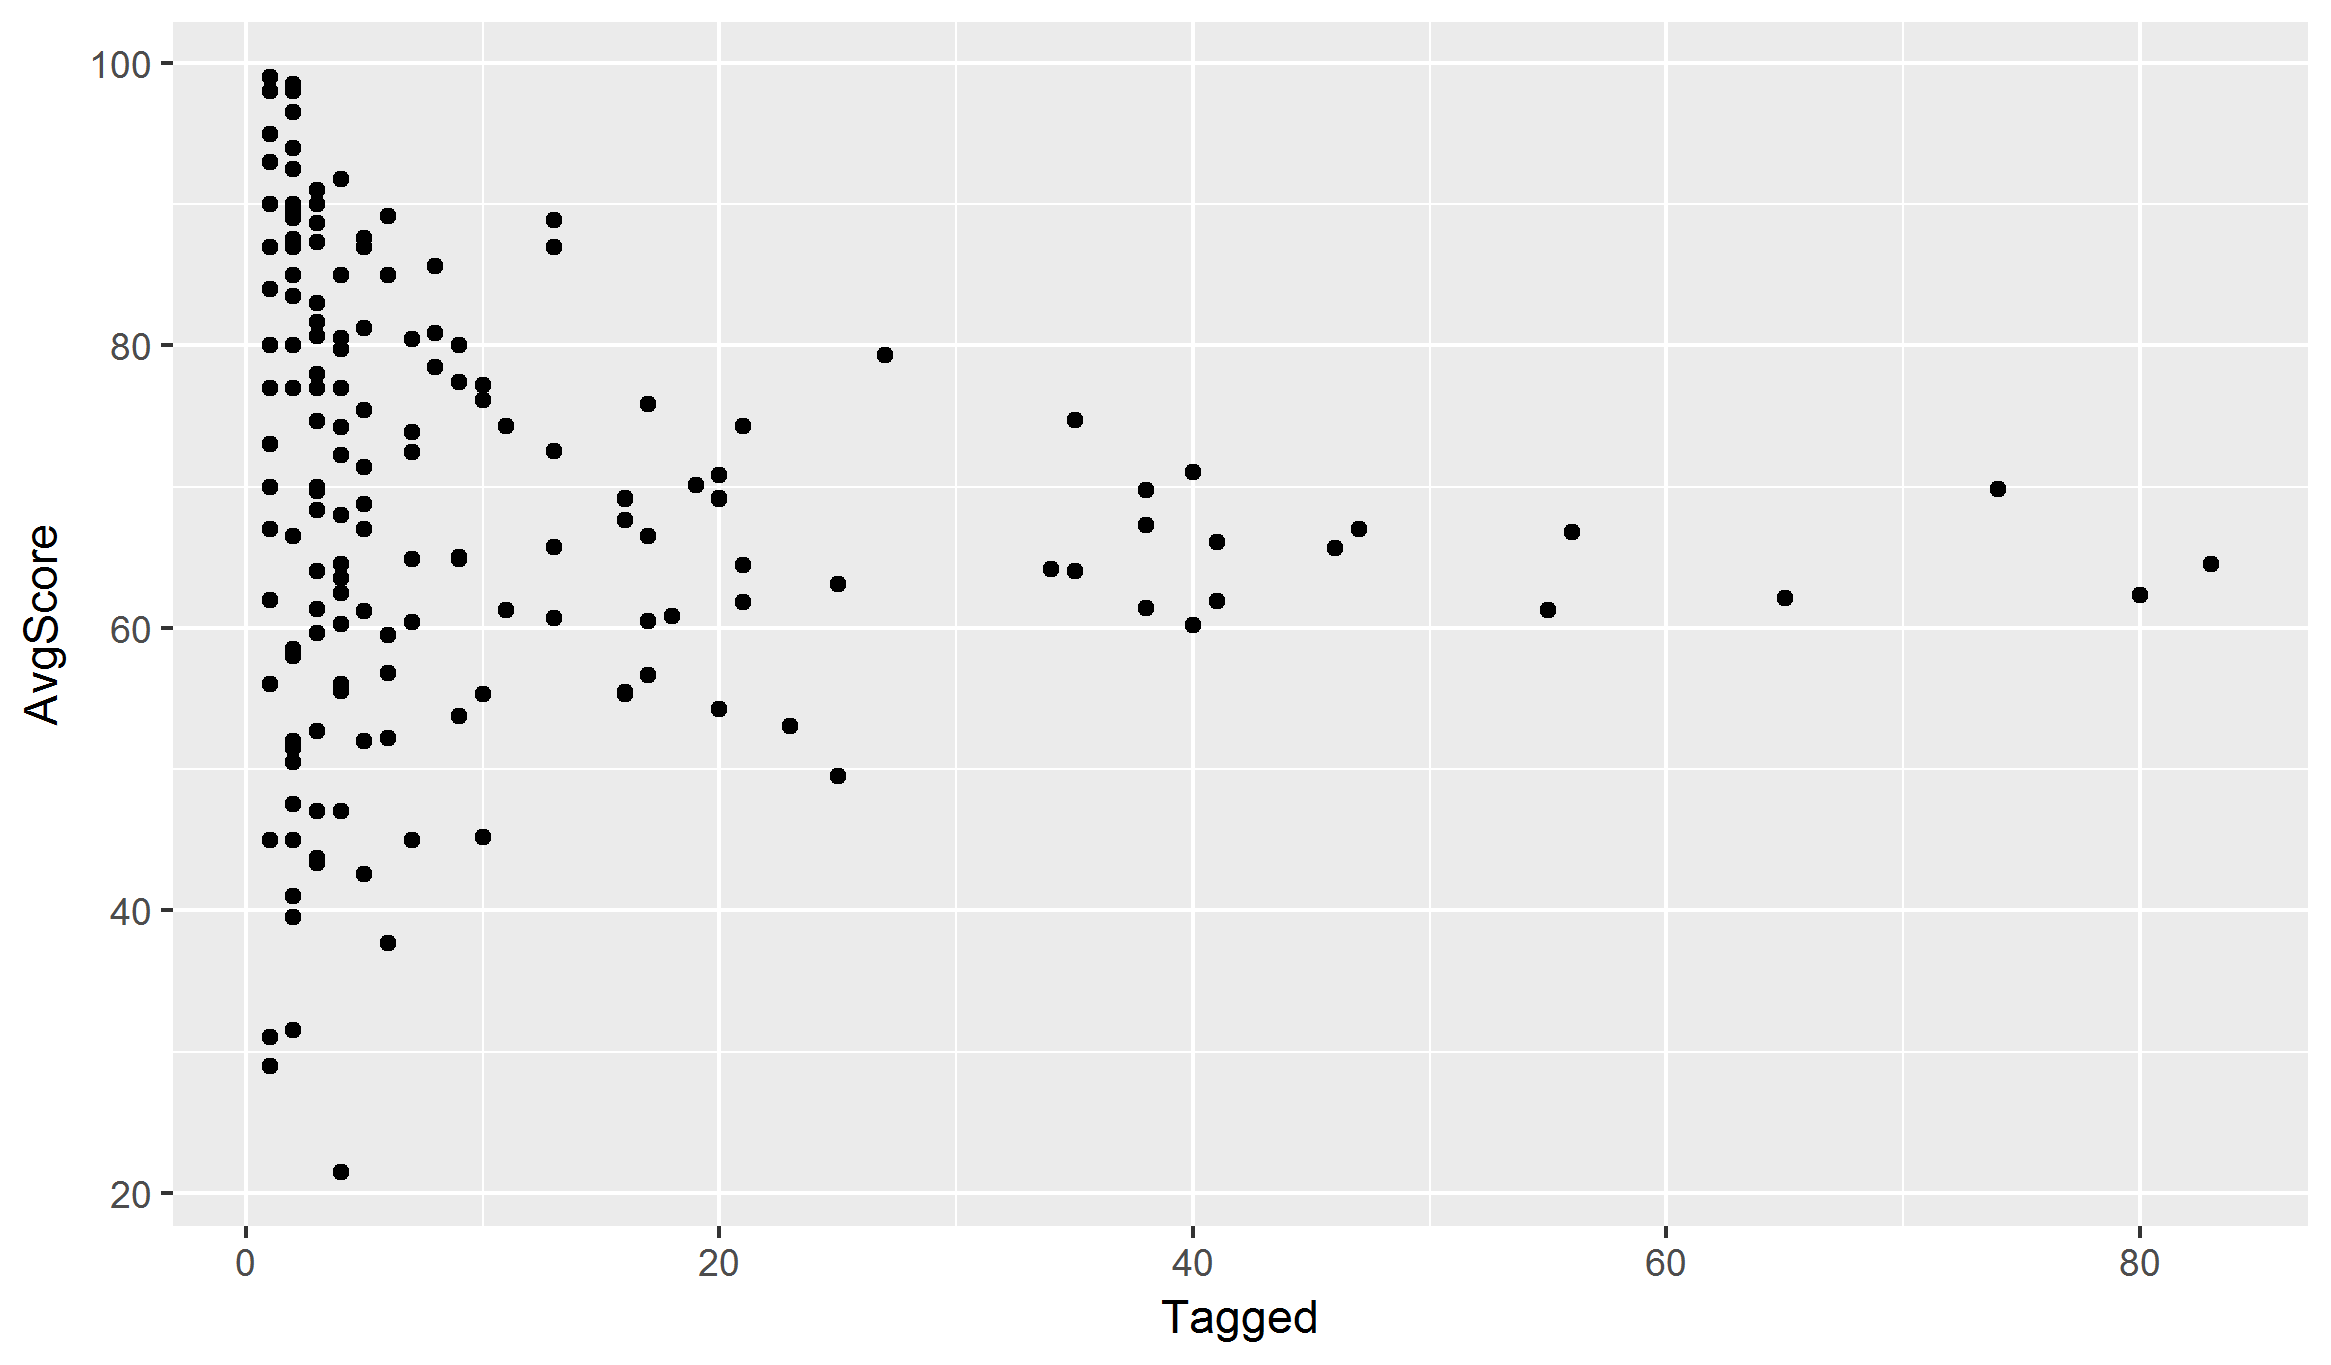
\includegraphics[width=\textwidth]{img/tag_score.png}
    \caption{Plotting of tags to scores}
    \label{fig:tag_score}
\end{figure}

\begin{figure}[H]
    \centering
    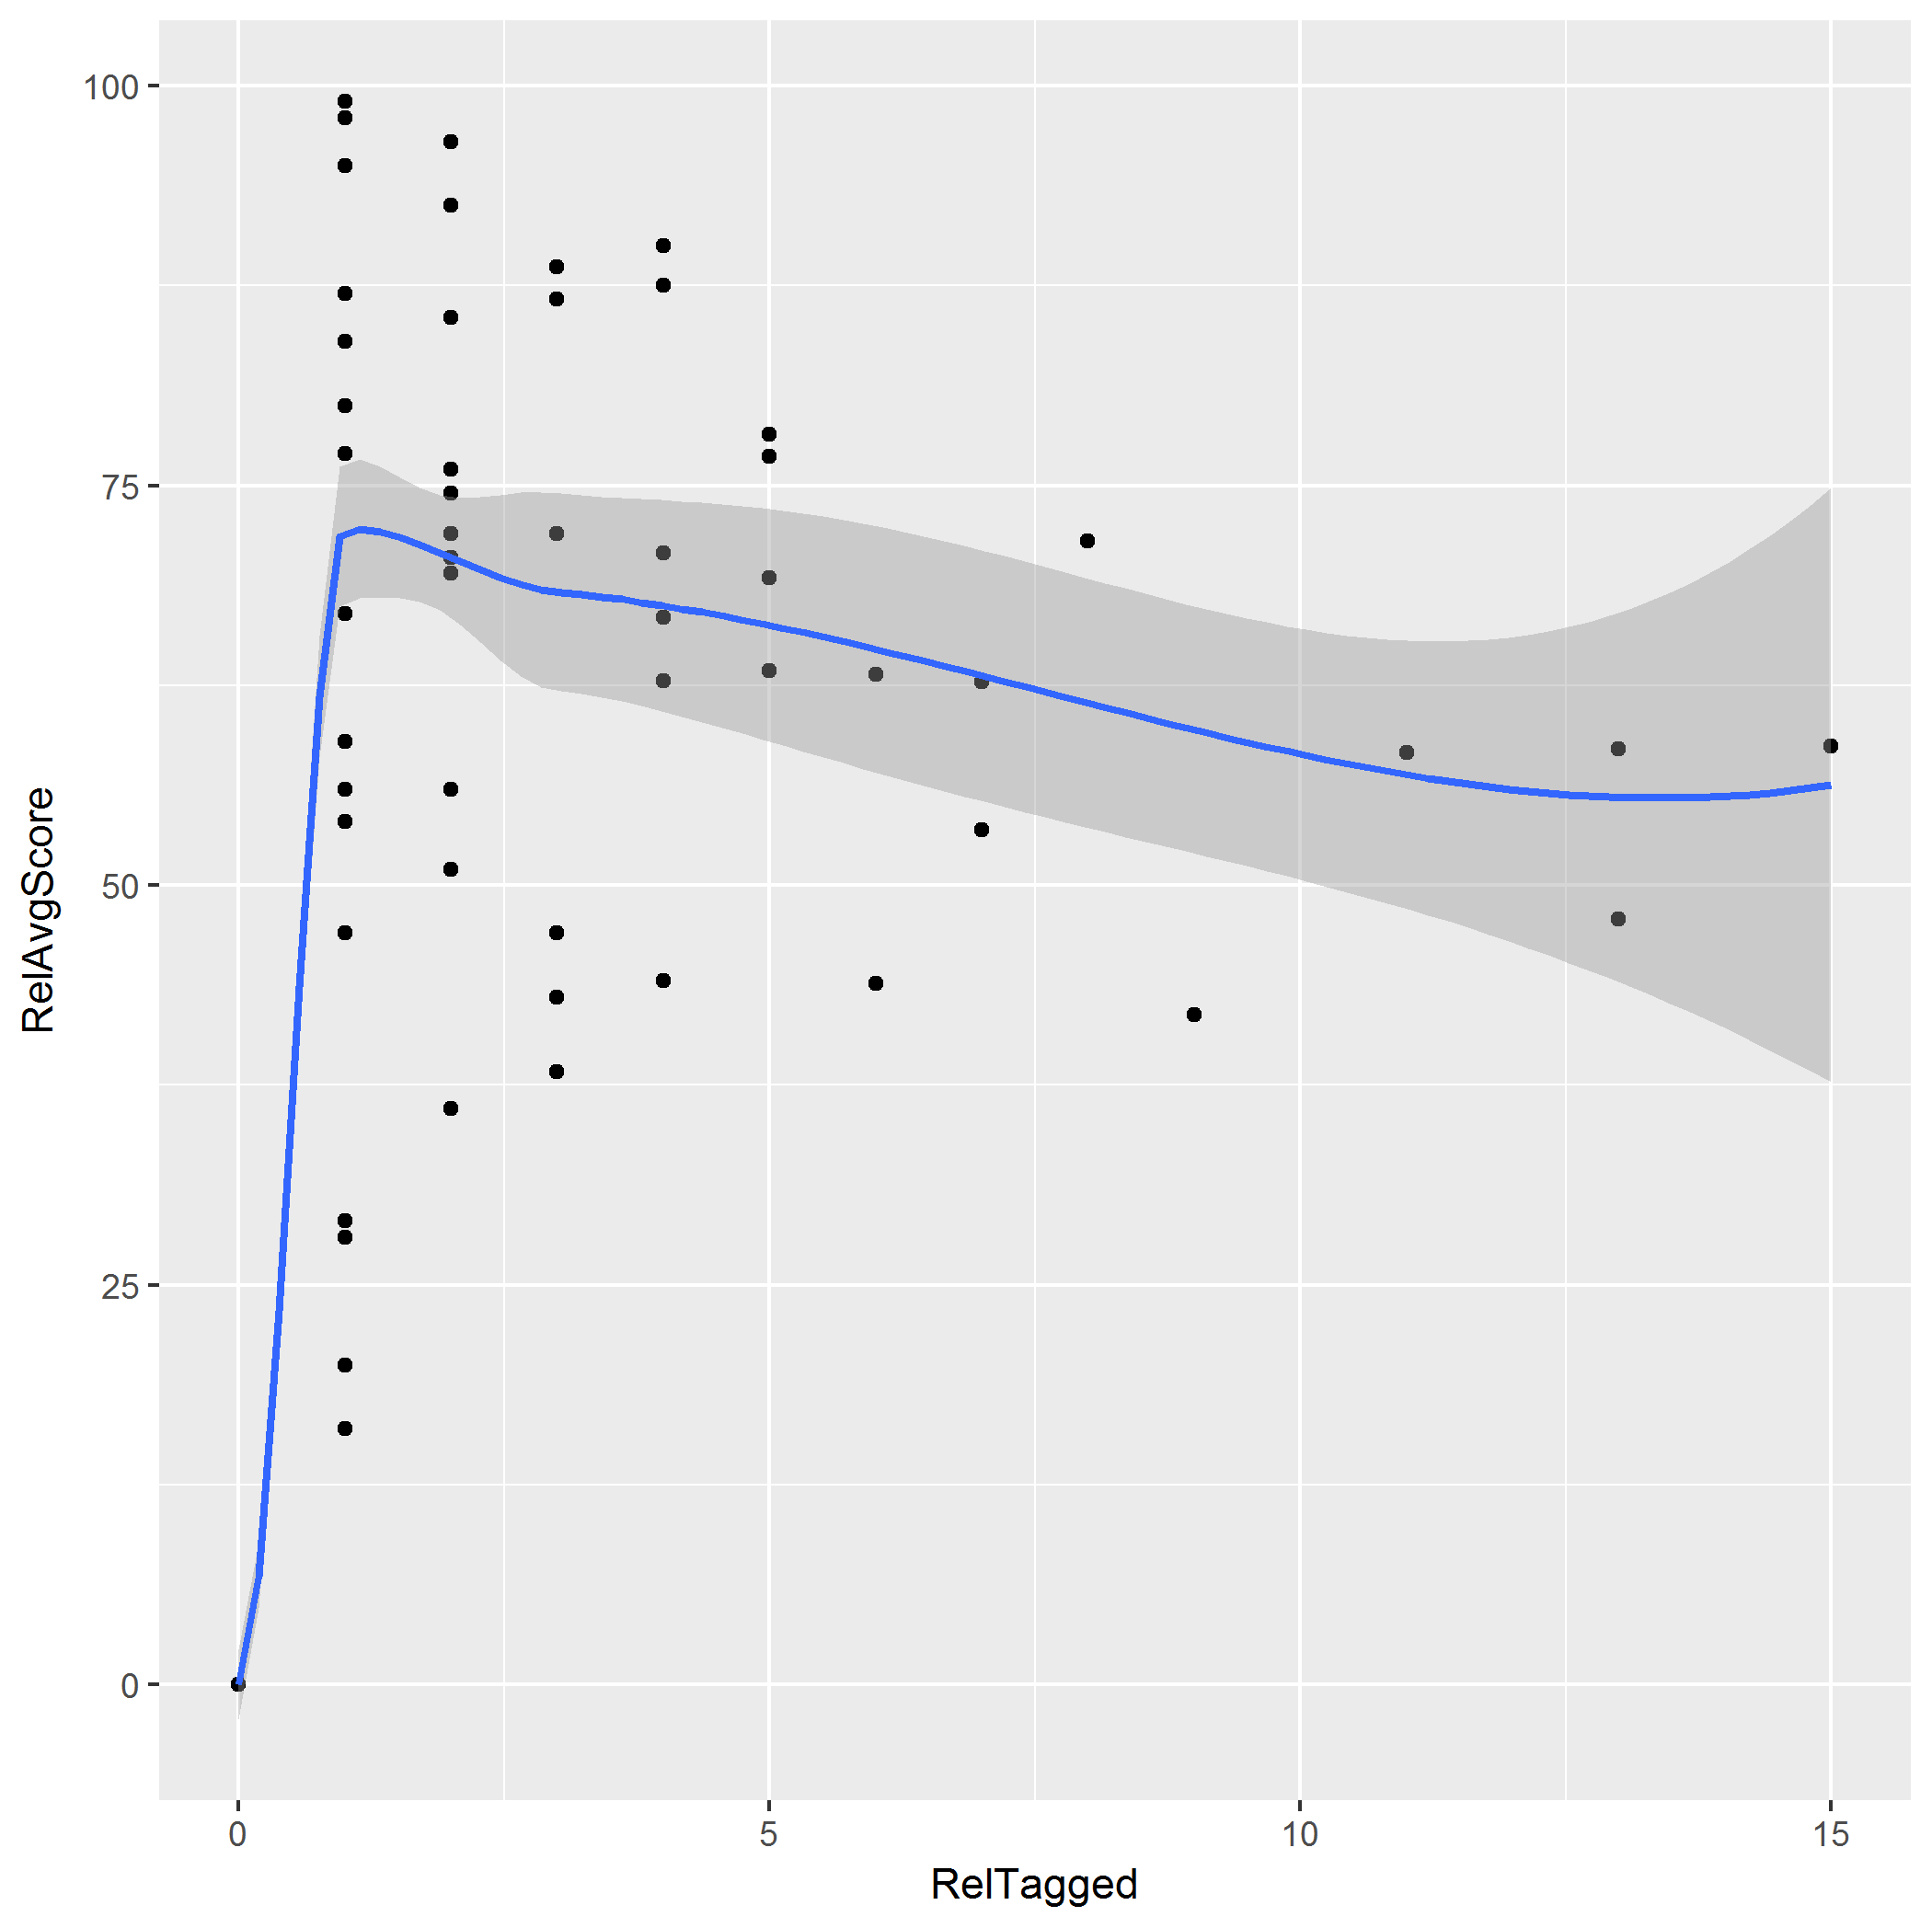
\includegraphics[width=\textwidth]{img/tag_score_rel.png}
    \caption{Plotting of relative tags to scores}
    \label{fig:tag_score_rel}
\end{figure}
% section figures_tables (end)
\end{document}